\section{Design Load Cases Review}
As mentioned in the last section, WEC design standards are emerging, with the recently released IEC TS 62600-2 \cite{IECTS62600-2} being the first such technical standard specific to WECs. Furthermore, guidelines and standards for related systems, such as ships and offshore structures, are also often applicable, as reviewed by \cite{Coe2017,WaveEnergyScotland2016}. However, it has not yet been clearly established when these guidelines may be used directly, and when WEC specific design methods must be further developed.

Design loads are the limiting load scenarios that define a WEC's structural strength requirements, and an accurate evaluation of the design load cases should enable an optimized structural design, ensure survival, and reduce overall WEC costs. Offshore structural design loads are evaluated for site specific environmental conditions; typically, characterized by the joint probability distribution of significant wave heights, Hs, and wave energy periods, Te. The probability of extreme sea states within the joint probability distribution is customarily indicated with contours of typical return periods, i.e. design life, such as 25, 50, 100 years (as illustrated in Figure \ref{fig:JPD}).

\begin{figure}[!t]
\centering
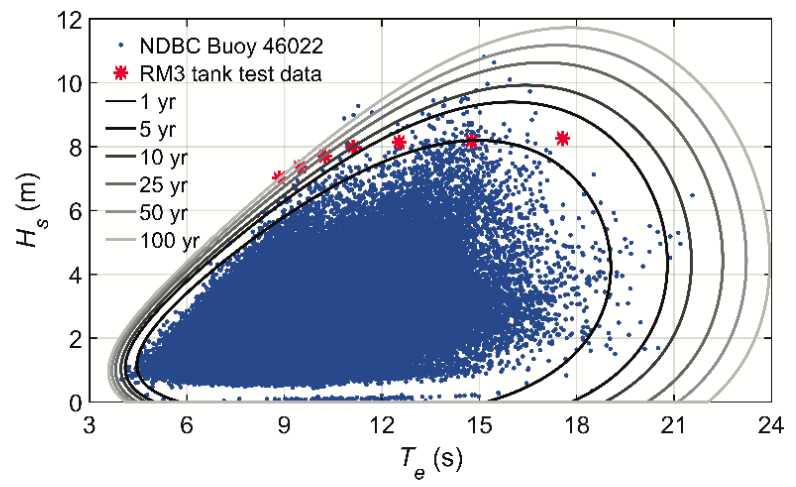
\includegraphics[width=0.65\textwidth]{./Figures/JPD.png}
\caption{Joint probability distribution for NDBC Buoy 46022.}
\label{fig:JPD}
\end{figure}

There are several prevailing methods for calculating design loads for a given wave environment. The simplest approach is the one-dimensional design load method, where loads are evaluated at the peak Hs on the selected design life contour for a range of Te (\cite{IECTS62600-2,N-003}). Alternatively, the contour design load method may be used, where loads are evaluated at intervals along the design life contour and the maximum response/load obtained is used as the design load (\cite{N-003,DNV-RP-C205}). Although the one-dimensional and contour design methods are typically applied in conjunction with correction or safety factors, implicit in both methods is the assumption that the design load is the same as the extreme wave condition load. Although this is often the case, it is not always true, particularly for WECs, which are designed for resonance at operational sea states. Alternatively, the most rigorous and accurate design method is the long-term, all sea-state contour approach. Using the all sea state method, short term extreme responses, typically 3 hrs, are obtained at points throughout the entire (Hs, Te) design space. The short-term responses are then weighted by their probabilities and summed to estimate the long- term design load for the specified design life (i.e. 25, 50, 100 yr). This method is clearly more arduous but has several advantages. First, power and fatigue loads, which typically must be calculated in the design process anyway, can be estimated using the same simulations. Second, no assumptions are made on where the design load conditions occur. Third, by obtaining the full sea state response surface, decisions on the WEC design life, survival modes, etc. are better informed. And finally, the all sea state approach can be used in conjunction with low- to mid-fidelity models to inform and reduce the computational expense of higher fidelity models to accurately determine the ultimate design loads.

While the design load methodology provides guidance on what sea states should be considered in calculating the design loads, it does not specify how these stochastic sea states should be realized. Irregular ocean waves are typically quantified in terms of a site specific empirical or idealized wave spectrum. As such, the most direct method of simulating a specified sea state, and a WEC's response to it, is to use the wave spectrum to create an irregular wave time series for the timeframe of interest. This approach, however, is often too computationally expensive when the timeframe of interest is on the order of 3 hr, particularly for high-fidelity models. Alternatively, assuming the wave heights follow a Rayleigh distribution, the extreme wave heights for a given sea state may be estimated with regular wave heights of H = 1.9Hs to approximate the maximum WEC responses (\cite{N-003}). Or, another simplified sea state realization approach, is the use a design, or focused wave; which uses broad-banded wave theory to define a series of wave amplitudes and phases that will produce the most-likely-extreme-response (MLER), as demonstrated by \cite{Quon2016}.

Irrespective of design load method, or sea state realization method, a modeling method is also necessary to simulate the sea state and the WEC response to the sea state. There are a wide range of modeling fidelities available. The simplest modeling approach is the linear frequency-domain, boundary-element- method (BEM)-based potential flow codes (e.g., WAMIT, Nemoh). Frequency-domain BEM codes calculate the hydrodynamic loads and resulting hydrodynamic coefficients based on linear radiation and diffraction theory. With this approach, the system dynamics are solved directly in the frequency domain, with simulation times often two orders of magnitude less than real time. At the next level of modeling fidelity are the linear time-domain, BEM-based codes, such as WEC-Sim (\cite{Yu2014a,Ruehl2014}). These types of models use the frequency-domain, BEM hydrodynamic coefficients to solve the system dynamics in the time domain and may also include weakly nonlinear quadratic damping, restoring and Froude-Krylov forcing terms. Simulation times for linear time-domain-type models are typically on the order of real time. To predict highly nonlinear effects, such as boundary layer viscous flow separation, turbulence, wave breaking, overtopping, etc., models based on the Navier-Stokes equations are generally employed. Navier- Stokes based computational fluid dynamics (CFD) have a large range of possible simulation times, roughly ~10$^4$-10$^8$ times real time, depending on the model complexity, particularly the turbulence model.

Potential combinations of design load method, sea state realization method, and modeling fidelity are summarized in Figure \ref{fig:DLM}. Each potential combination is valid but may make more, or less, sense depending on the design stage and modeling resources available. For example, it would be reasonable to use a one-dimensional design load method, with regular wave sea state realizations, along with a BEM model, to obtain proof-of- concept estimates in the initial stages of a WEC design. However, in the latter stages of design, where extremely accurate design loads must be obtained, a full sea state design load method, with irregular wave timeseries realizations, utilizing high fidelity CFD would be highly desirable. Unfortunately, this combination of design load analysis methods is currently far too computationally expensive and time consuming to be feasible. Because of this computational limitation, an extreme condition/ design load analysis framework has been loosely suggested in the past for analyzing WEC design loads (\cite{Quon2016,VanRij2017,Coe2016,VanRij2017a}). The crux of this framework is to use low- to mid-fidelity models to inform high-fidelity models, such that accurate design loads may be obtained, without having to perform a full long-term, all sea state loads analysis using high-fidelity models.

\begin{figure}[!t]
\centering
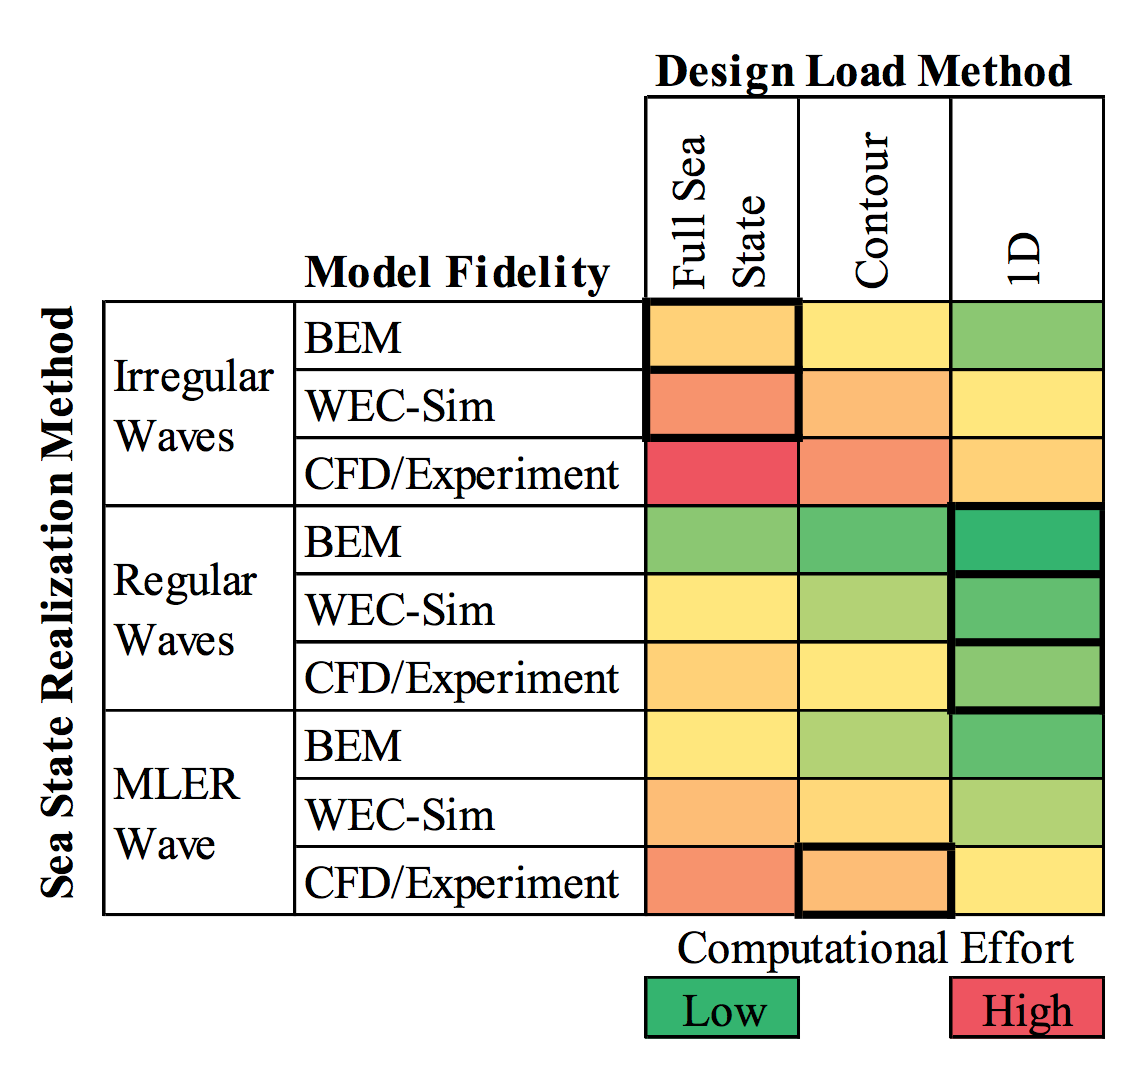
\includegraphics[width=0.55\textwidth]{./Figures/DLM.png}
\caption{Design load analysis approaches and their relative computational efficiency.}
\label{fig:DLM}
\end{figure}
